
\section{Wasserfalldiagramm}
\label{section:wasserfall}
\begin{frame}%STARTCONTENT

\frametitle{Empfang}
\begin{itemize}
  \item Frequenz wird am Funkgerät über Drehknopf oder Tasten eingestellt
  \item Es können nur Stationen auf der eingestellten Frequenz gehört werden
  \item Langsam \enquote{über das Band drehen}, um andere Stationen zu hören
  \end{itemize}
\end{frame}

\begin{frame}
\frametitle{Amplitudenspektrum und Wassefalldiagramm}
\begin{columns}
    \begin{column}{0.48\textwidth}
    
\begin{figure}
    \includegraphics[width=0.85\textwidth]{foto/95}
    \caption{\scriptsize Display eines ICOM IC-9700 mit Frequenzanzeige, Amplitudenspektrum und Wasserfalldiagramm. Eine starke Station wird empfangen.}
    \label{n_wasserfall_starke_station}
\end{figure}

    \end{column}
   \begin{column}{0.48\textwidth}
       \begin{itemize}
  \item Moderne Funkgeräte
  \item Anzeige weiterer sendender Stationen ober- und unterhalb der eingestellten Frequenz
  \end{itemize}

   \end{column}
\end{columns}

\end{frame}

\begin{frame}
\frametitle{Amplitudenspektrum}
\begin{columns}
    \begin{column}{0.48\textwidth}
    
\begin{figure}
    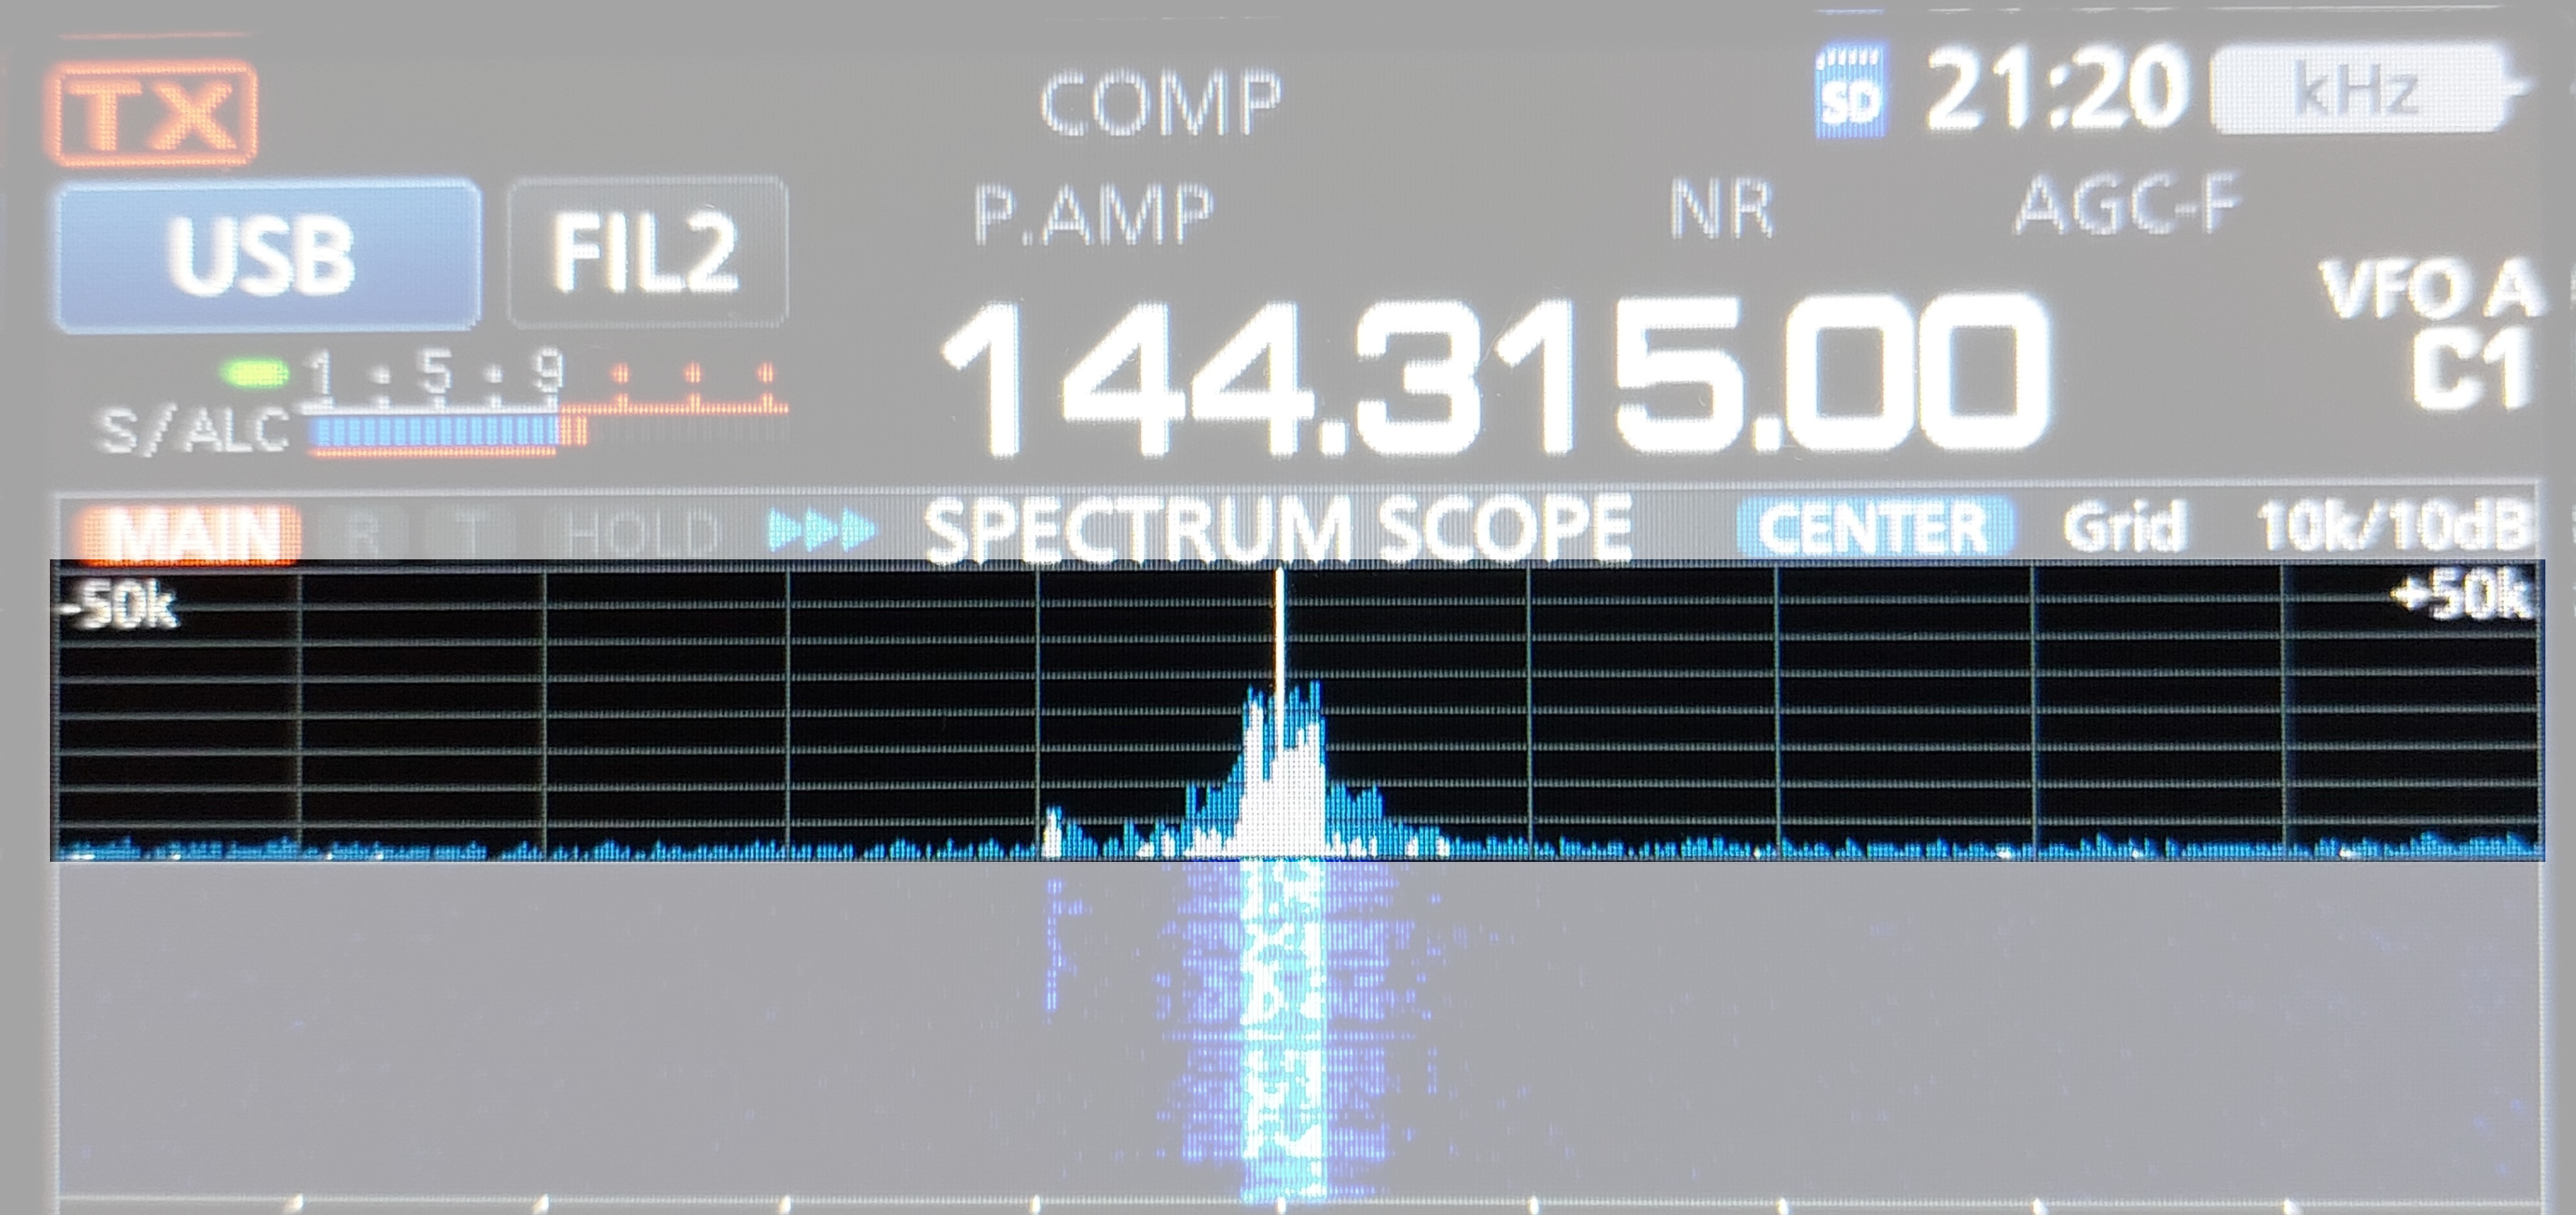
\includegraphics[width=0.85\textwidth]{foto/135}
    \caption{\scriptsize Display eines ICOM IC-9700. Hervorgehoben ist das Amplitudenspektrum}
    \label{n_wasserfall_amplitudenspektrum}
\end{figure}

    \end{column}
   \begin{column}{0.48\textwidth}
       \begin{itemize}
  \item Amplitude umso höher je stärker das Signal ist
  \item Weitere Stationen sind im Amplitudenspektrum sichtbar
  \end{itemize}

   \end{column}
\end{columns}

\end{frame}

\begin{frame}
\frametitle{Wasserfalldiagramm}
\begin{columns}
    \begin{column}{0.48\textwidth}
    
\begin{figure}
    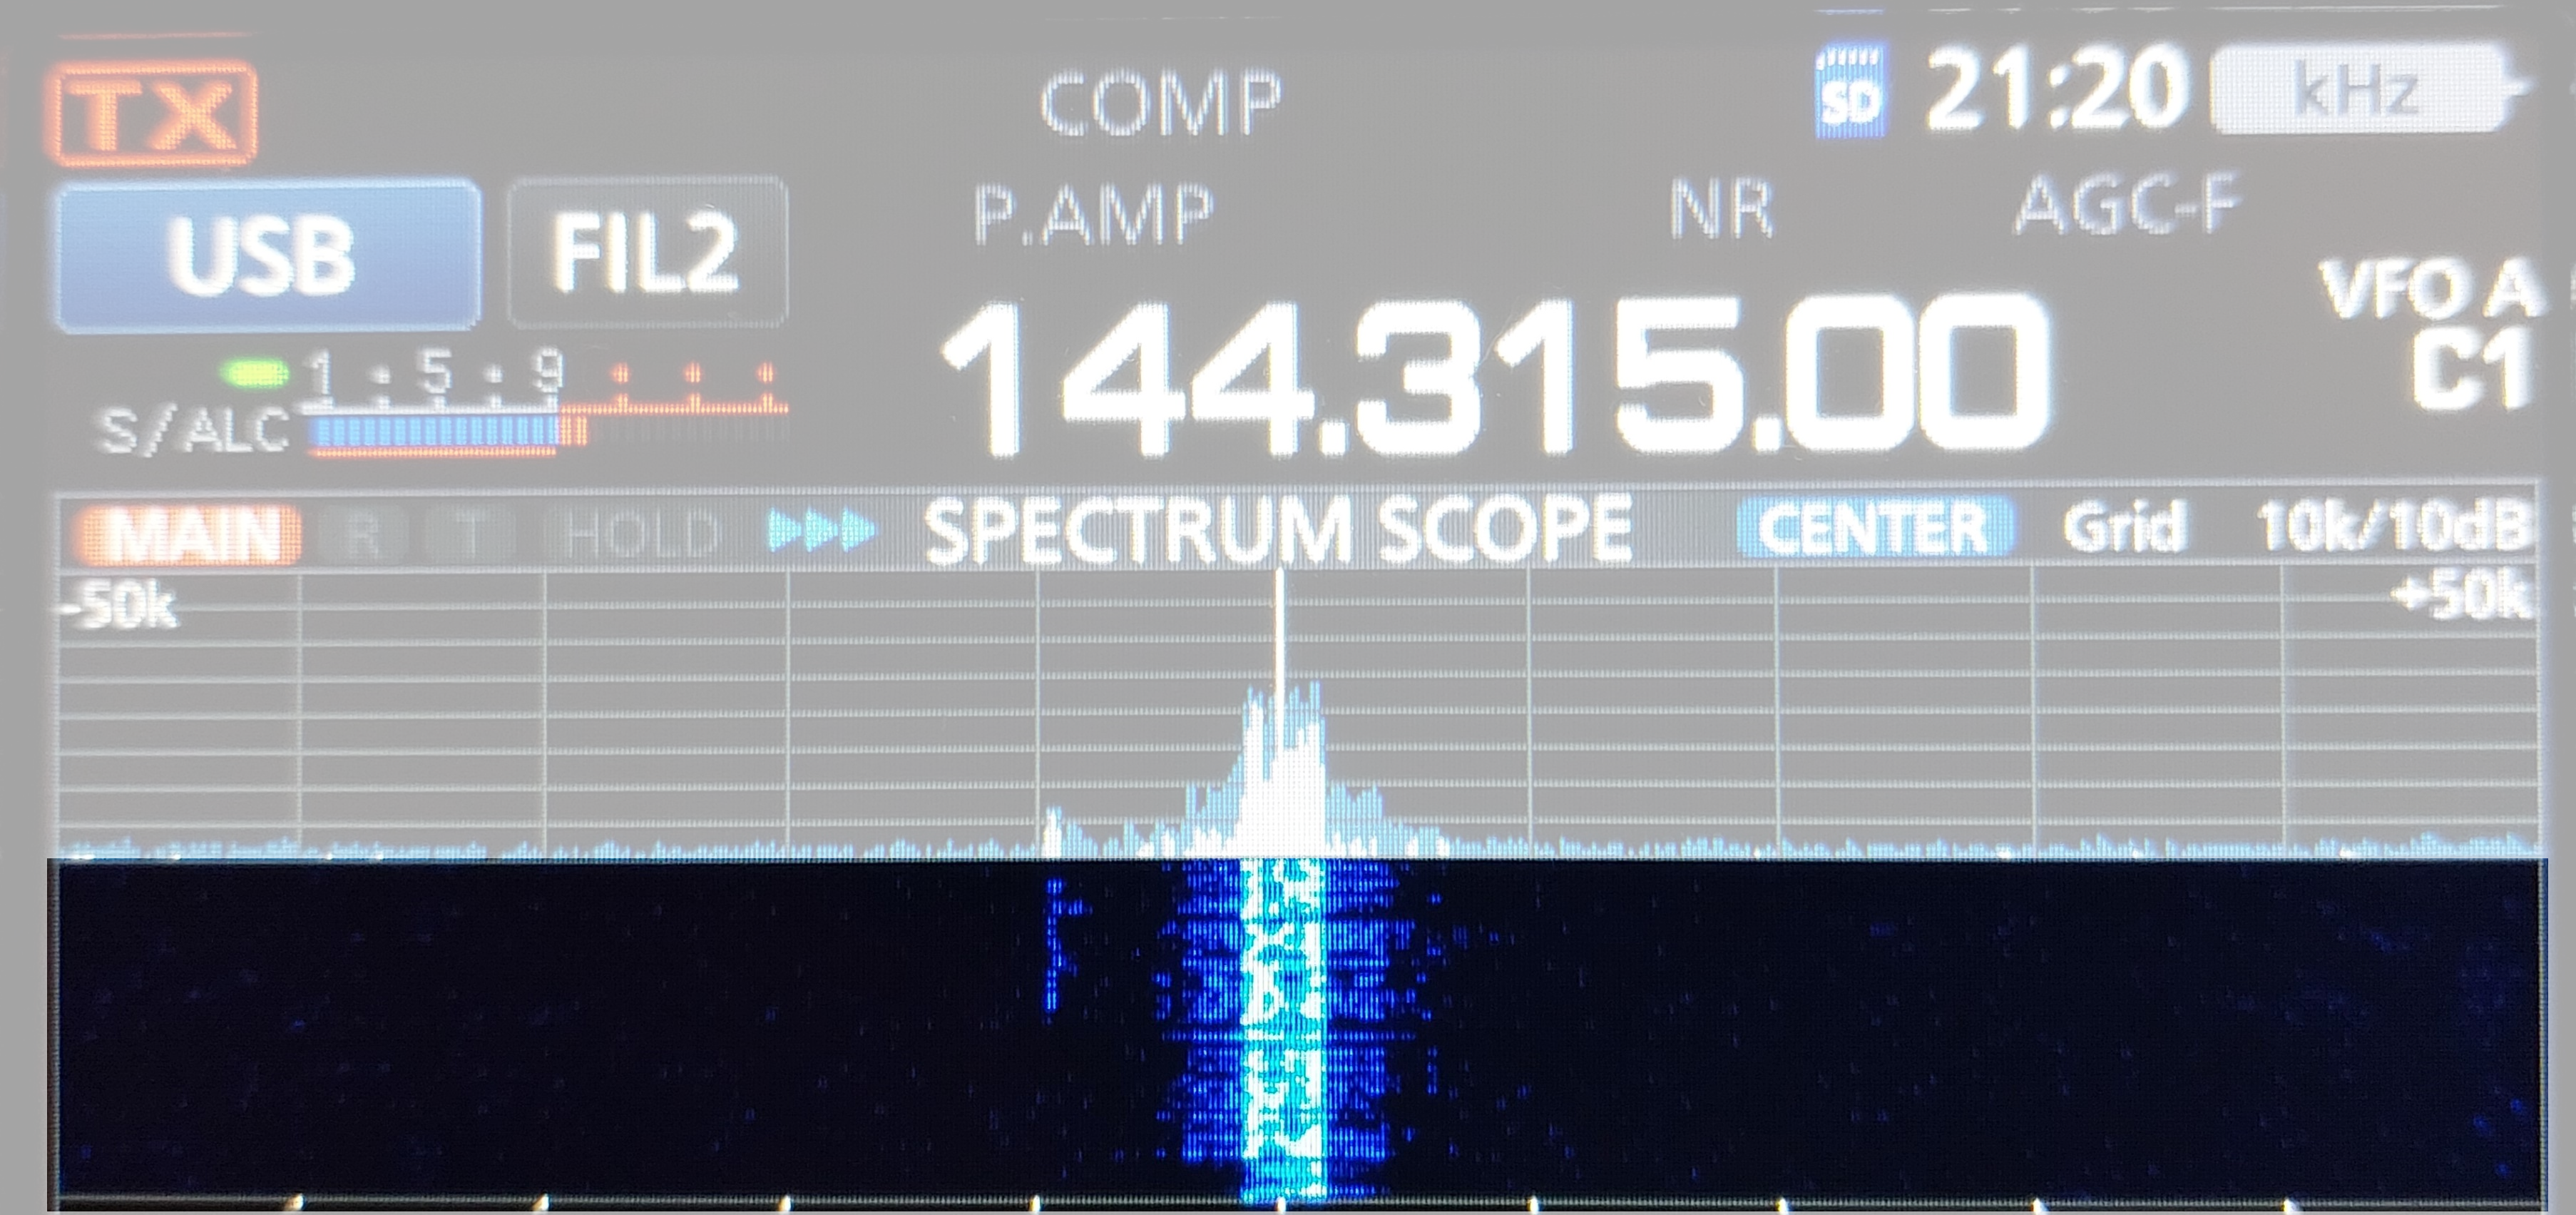
\includegraphics[width=0.85\textwidth]{foto/136}
    \caption{\scriptsize Display eines ICOM IC-9700. Hervorgehoben ist der Wasserfall}
    \label{n_wasserfall_wasserfall}
\end{figure}

    \end{column}
   \begin{column}{0.48\textwidth}
       \begin{itemize}
  \item Zeitlicher Verlauf auf senkrechter Achse
  \item Farbton oder Helligkeit zeigt die Stärke des Signals
  \item Läuft von oben nach unten durch
  \item Beginn und Ende einer Aussendung erkennbar
  \end{itemize}

   \end{column}
\end{columns}

\end{frame}

\begin{frame}
\only<1>{
\begin{PQuestion}{NF104}{Die Darstellung zeigt das Display eines Transceivers. Wie wird die Anzeige 3 bezeichnet?}{Power-Meter}
{Amplitudenspektrum}
{S-Meter}
{Wasserfalldiagramm}
{\DARCimage{1.0\linewidth}{578include}}\end{PQuestion}

}
\only<2>{
\begin{PQuestion}{NF104}{Die Darstellung zeigt das Display eines Transceivers. Wie wird die Anzeige 3 bezeichnet?}{Power-Meter}
{\textbf{\textcolor{DARCgreen}{Amplitudenspektrum}}}
{S-Meter}
{Wasserfalldiagramm}
{\DARCimage{1.0\linewidth}{578include}}\end{PQuestion}

}
\end{frame}

\begin{frame}
\only<1>{
\begin{PQuestion}{NF105}{Die Darstellung zeigt das Display eines Transceivers. Wie wird die Anzeige 4 bezeichnet?}{Regenbogendiagramm}
{Wasserfalldiagramm}
{SWR-Meter}
{Power-Meter}
{\DARCimage{1.0\linewidth}{578include}}\end{PQuestion}

}
\only<2>{
\begin{PQuestion}{NF105}{Die Darstellung zeigt das Display eines Transceivers. Wie wird die Anzeige 4 bezeichnet?}{Regenbogendiagramm}
{\textbf{\textcolor{DARCgreen}{Wasserfalldiagramm}}}
{SWR-Meter}
{Power-Meter}
{\DARCimage{1.0\linewidth}{578include}}\end{PQuestion}

}
\end{frame}

\begin{frame}
\only<1>{
\begin{PQuestion}{NF106}{Die Darstellung zeigt das Display eines Transceivers. Was wird im Wasserfalldiagramm dargestellt und wie erfolgt die Darstellung?}{Frequenz und Zeit auf den Achsen und Signalstärke als Farbton und/oder Helligkeit.}
{Frequenz und Signalstärke auf den Achsen und Zeit als Farbton und/oder Helligkeit.}
{Signalstärke und Zeit auf den Achsen und Frequenz als Farbton und/oder Helligkeit.}
{Signalstärke und Phase auf den Achsen und Zeit als Farbton und/oder Helligkeit.}
{\DARCimage{1.0\linewidth}{579include}}\end{PQuestion}

}
\only<2>{
\begin{PQuestion}{NF106}{Die Darstellung zeigt das Display eines Transceivers. Was wird im Wasserfalldiagramm dargestellt und wie erfolgt die Darstellung?}{\textbf{\textcolor{DARCgreen}{Frequenz und Zeit auf den Achsen und Signalstärke als Farbton und/oder Helligkeit.}}}
{Frequenz und Signalstärke auf den Achsen und Zeit als Farbton und/oder Helligkeit.}
{Signalstärke und Zeit auf den Achsen und Frequenz als Farbton und/oder Helligkeit.}
{Signalstärke und Phase auf den Achsen und Zeit als Farbton und/oder Helligkeit.}
{\DARCimage{1.0\linewidth}{579include}}\end{PQuestion}

}
\end{frame}

\begin{frame}
\frametitle{Unterschied Oszillogramm und Amplitudenspektrum}
\begin{itemize}
  \item Amplitudenspektrum zeigt horizontal Amplituden für verschiedene Frequenzen an
  \item Oszillogramm zeigt horizontal Amplituden zu verschiedenen Zeitpunkten an
  \end{itemize}
\end{frame}

\begin{frame}
\only<1>{
\begin{QQuestion}{NI401}{Was ist der Unterschied zwischen einem Oszillogramm und einem Amplitudenspektrum?}{Ein Oszillogramm zeigt den Strom und ein Amplitudenspektrum die Spannung eines Signals.}
{Ein Oszillogramm zeigt die Frequenzanteile und ein Amplitudenspektrum einen zeitlichen Verlauf eines Signals.}
{Ein Oszillogramm zeigt die Spannung und ein Amplitudenspektrum den Strom eines Signals.}
{Ein Oszillogramm zeigt einen zeitlichen Verlauf und ein Amplitudenspektrum die Frequenzanteile eines Signals.}
\end{QQuestion}

}
\only<2>{
\begin{QQuestion}{NI401}{Was ist der Unterschied zwischen einem Oszillogramm und einem Amplitudenspektrum?}{Ein Oszillogramm zeigt den Strom und ein Amplitudenspektrum die Spannung eines Signals.}
{Ein Oszillogramm zeigt die Frequenzanteile und ein Amplitudenspektrum einen zeitlichen Verlauf eines Signals.}
{Ein Oszillogramm zeigt die Spannung und ein Amplitudenspektrum den Strom eines Signals.}
{\textbf{\textcolor{DARCgreen}{Ein Oszillogramm zeigt einen zeitlichen Verlauf und ein Amplitudenspektrum die Frequenzanteile eines Signals.}}}
\end{QQuestion}

}
\end{frame}%ENDCONTENT
